
\chapter{Konzept}
\label{sec:konzept}

\section{Mockups}
Der Buchungsprozess vom Hotel und Flug Produkt von travel.ch benötigt drei Ansichten, für welche hier Mockups aufgezeigt werden.
Diese wurden mit dem UI Designer von Bonita erstellt (siehe \cref{sec:analyse:bonita:forms:forms} \nameref{sec:analyse:bonita:forms:forms}).

\begin{figure}[H]
	\centering
	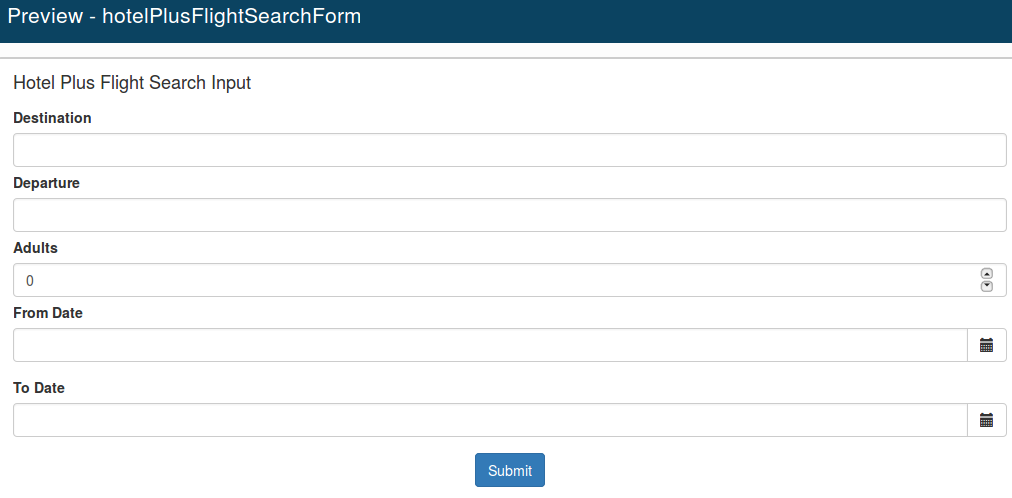
\includegraphics[width=1\textwidth]{images/forms-search.png}
	\caption{Suchformular Mockup}
	\label{fig:konzept:mockups:search}
\end{figure}

Das Suchformular ist vereinfacht dargestellt. Für die Destination muss man einen gültigen Namen eingeben. Auf der Webseite travel.ch wird dem User beim Tippen Vorschläge angezeigt. Dies wurde für dieses Projekt nicht umgesetzt.

Für die Passagiere kann im obigen Formular nur eine Anzahl für die Erwachsenen angegeben werden. Kinder können nicht angewählt werden, da für diese zusätzlich noch das Geburtsdatum angegeben werden muss. Auch die Wahl nach mehreren Zimmern ist nicht möglich. Für die Anzahl der Erwachsenen wird ein Hotelzimmer gesucht.

\begin{figure}[H]
	\centering
	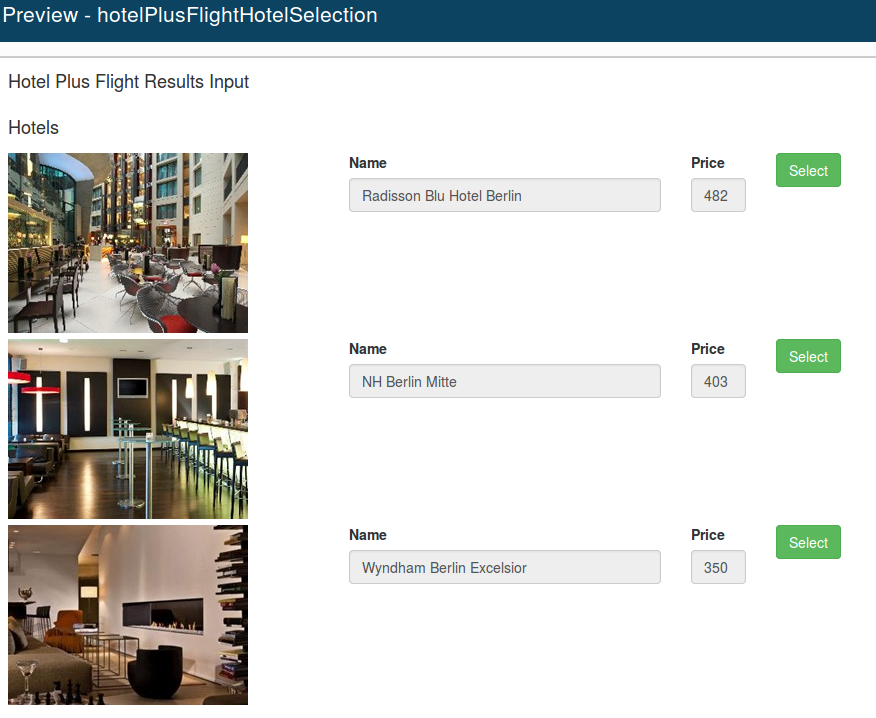
\includegraphics[width=1\textwidth]{images/forms-select-hotel.png}
	\caption{Mockup für die Hotel Suchresultate}
	\label{fig:konzept:mockups:selecthotel}
\end{figure}
Diese Ansicht zeigt ein Foto des Hotels, dessen Namen und der günstigste Preis. Von der \Gls{glos:api} werden noch mehrere Fotos, eine Geokoordinate für die Anzeige einer Maps, Bewertungsdaten, etc. übermittelt. Diese Informationen werden jedoch nicht angezeigt.

\begin{figure}[H]
	\centering
	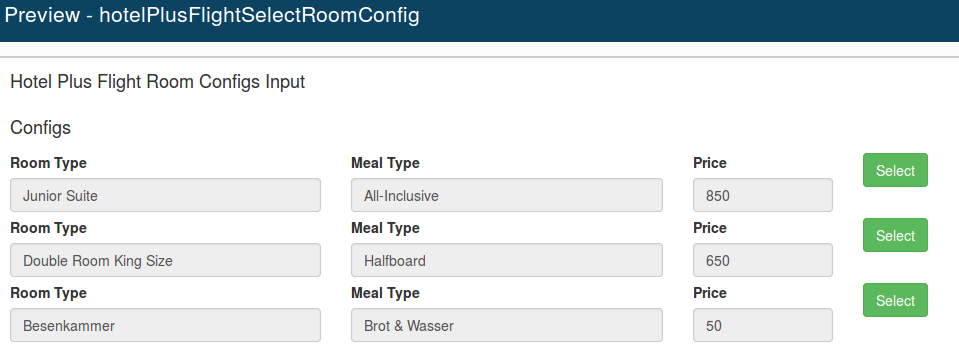
\includegraphics[width=1\textwidth]{images/forms-select-roomconfig.png}
	\caption{Mockup für die Hotelzimmer Konfiguration}
	\label{fig:konzept:mockups:selectroomconfig}
\end{figure}
Auf der travel.ch Seite werden die Zimmer-Konfigurationen als Matrix dargestellt. Die Zeilen sind die Zimmer-, und die Spalten die Verpflegungstypen. In Bonita ist dies jedoch nur sehr umständlich abbildbar. Deshalb wurde die Ansicht vereinfacht und als Liste dargestellt.

Im \cref{sec:analyse:api} \nameref{sec:analyse:api} wurden die verschiedenen API